% =============== IHM ===============
\chapter{IHM}

% ------------- Interface de l'écran d'accueil ------------
\section{Interface de l'écran d'accueil}
	Lorsque l'utilisateur lance le programme, celui-ci est dirigé vers un écran d'accueil.

	\color{red}
	Cette écran est divisé en deux parties principales.

	La première, à gauche, est la partie où l'utilisateur a la possibilité de développer sa propre Intelligence Artificielle (IA). L'utilisateur doit coder impérativement en Java sinon la compilation ne fonctionnera pas.

	La deuxième, à droite, est la partie liée au jeu. Une description détaillée des règles du jeu figure en haut de l'écran afin que l'utilisateur novice puisse très vite prendre ses marques.

	\color{black}
	Avant de créer ou rejoindre une partie, l'utilisateur doit renseigner un pseudo. Ce pseudo sera son identifiant lors des parties. De plus, il pourra choisir d'envoyer son IA, qu'il aura développé au préalable, dans le labyrinthe ou bien de jouer manuellement au jeu. Une fois que l'utilisateur aura rentré ces paramètres, il peut choisir de rejoindre une partie ou d'en créer une. S'il choisit d'en créer une il devra renseigner le nombre maximum de joueurs que la partie pourra accueillir.

	Le choit de jouer avec une IA ou manuellement se fera à l'aide de radios boutons qui mettra en surbrillance le choix de l'utilisateur.

	La figure~\ref{fig:ecran_accueil} représente une maquette de l'écran d'accueil.
	\begin{figure}[h]
		\centering
		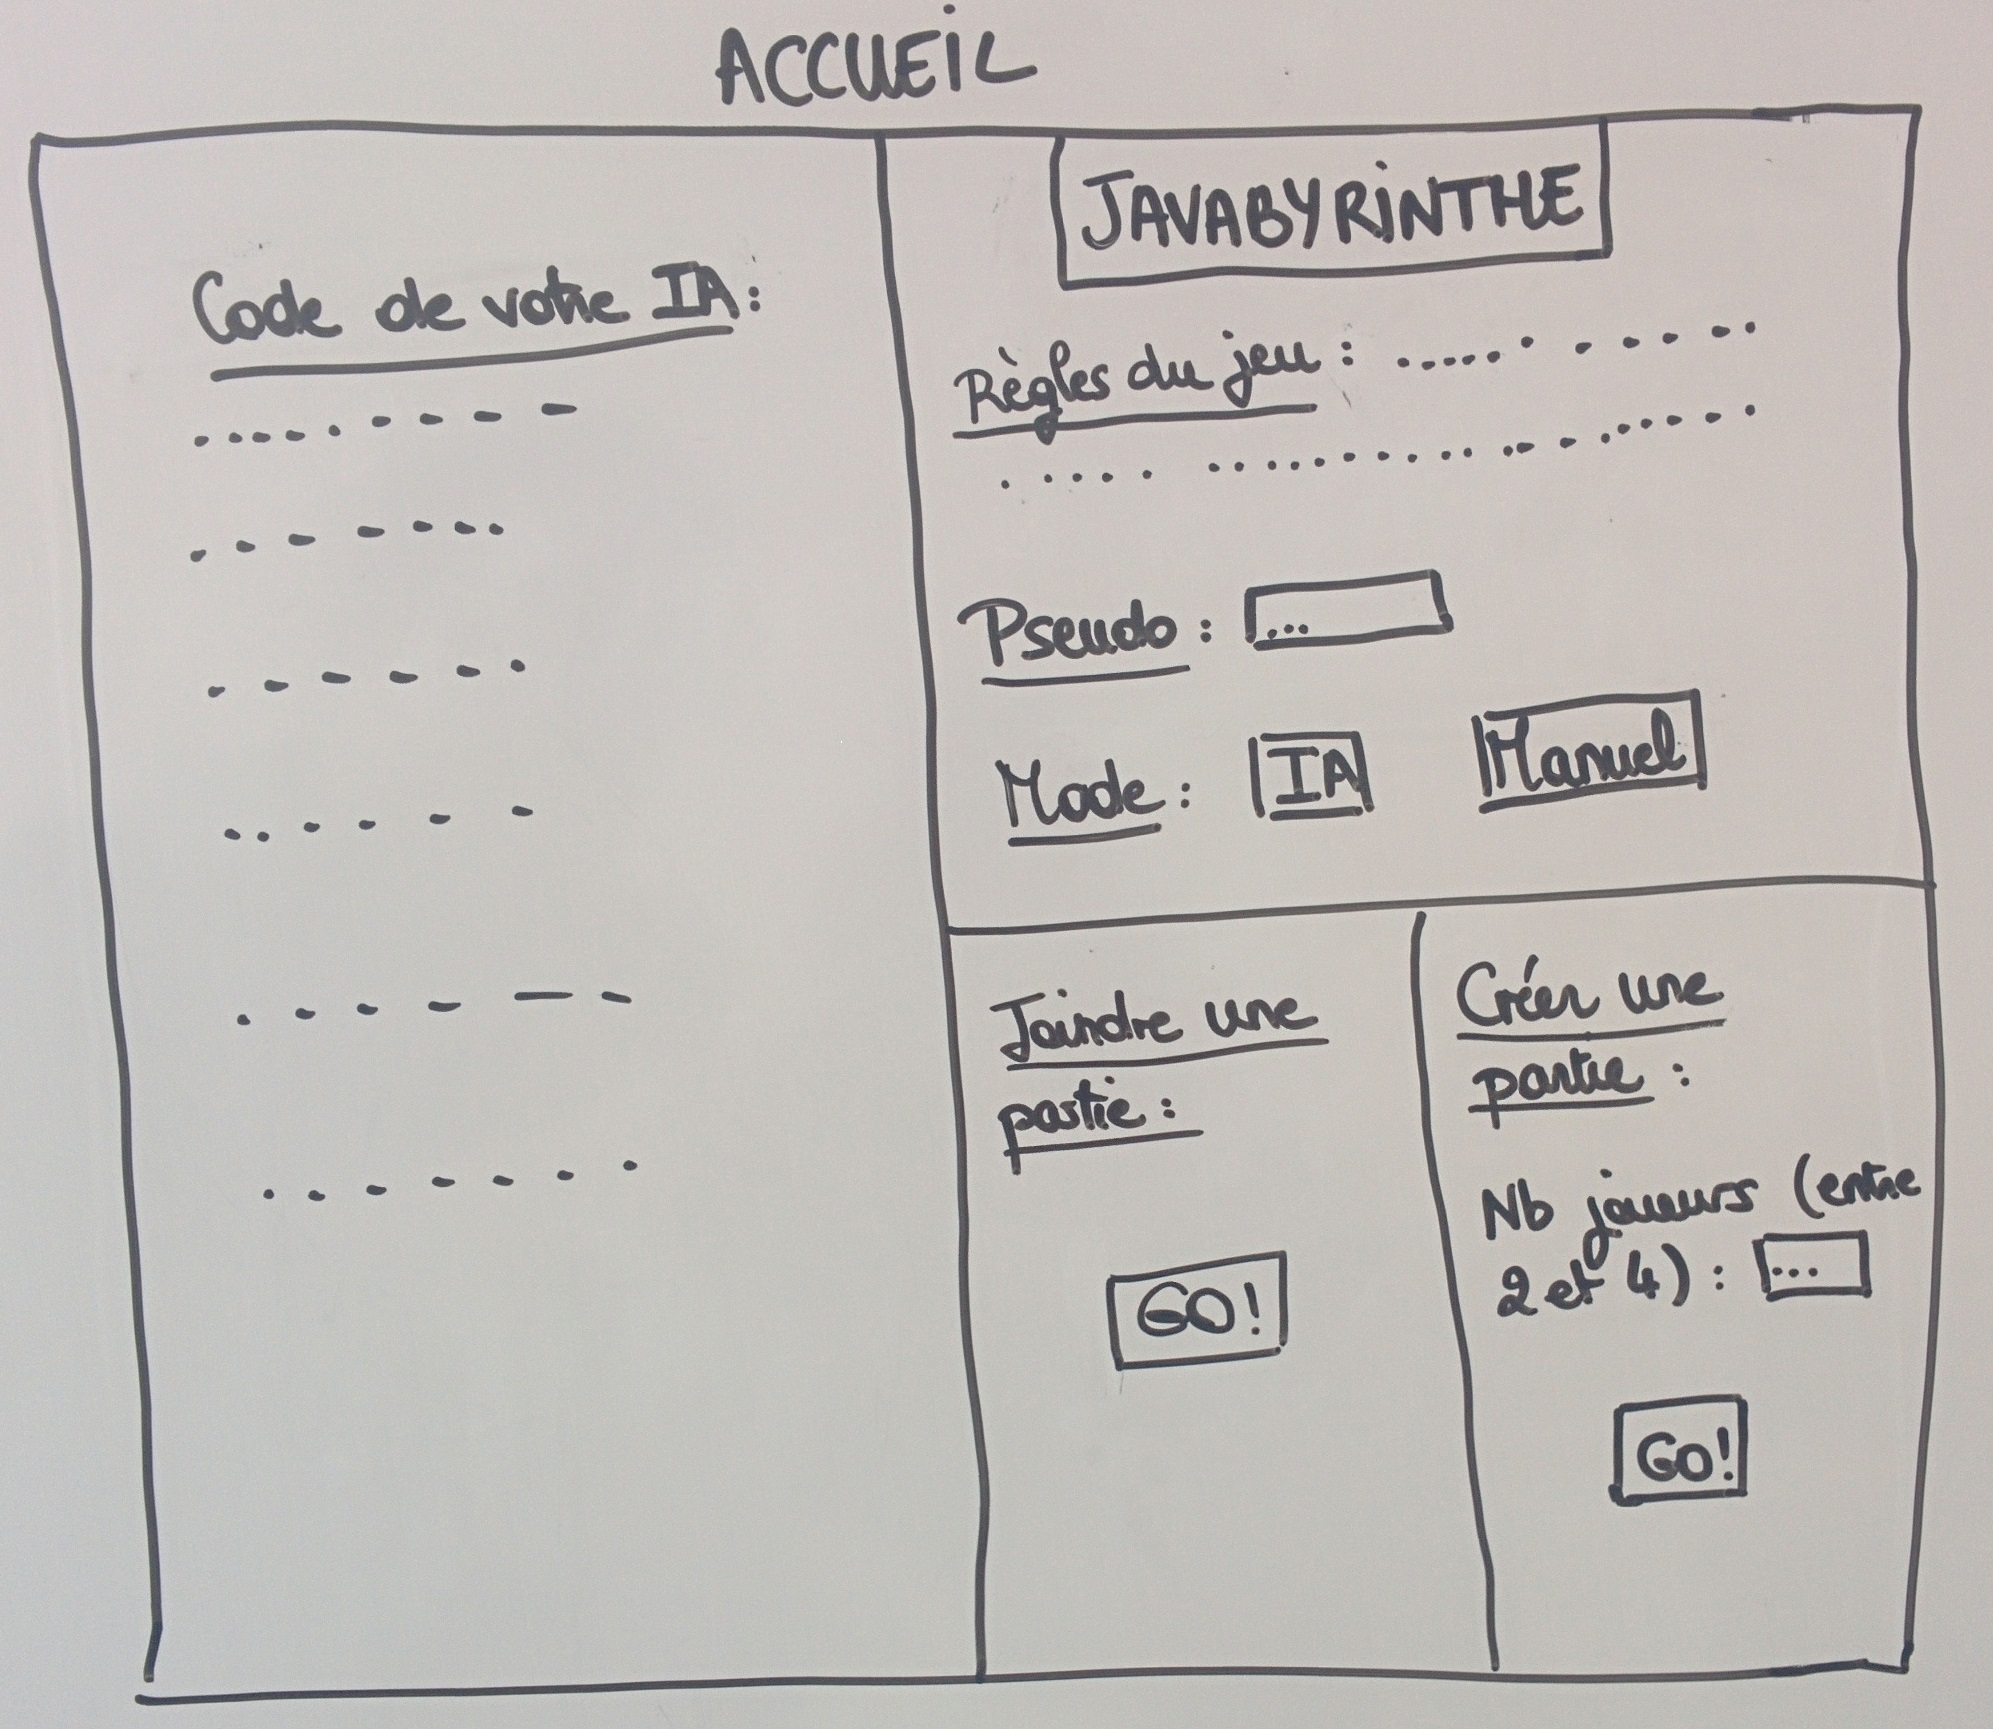
\includegraphics[width=15cm]{images/schema_ecran_accueil.jpg}
		\caption{Schéma de l'écran d'accueil}
		\label{fig:ecran_accueil}
	\end{figure}

	% ------------- Gestion des parties ------------
	\subsection{Gestion des parties}
		Comme décrit précédemment, l'utilisateur doit compléter tous les paramètres avant de pouvoir jouer. Si les paramètres ne sont que partiellement remplis ou non conforme l'utilisateur ne pourra pas jouer et un message d'erreur sera affiché. Une fois que l'utilisateur a tout rempli correctement, il doit choisir entre rejoindre ou créer une partie.

		S'il choisit de rejoindre une partie, l'utilisateur sera redirigé directement vers la première partie avec des places disponibles. Aucun choix de partie ne sera mis en place afin de faciliter la gestion des salles.

		S'il choisit de créer une partie, il doit renseigner le nombre de joueurs maximums et cliquer ensuite sur \textit{GO!}. Si le nombre de joueur n'est pas compris entre 2 et 4 inclus, un message d'erreur sera affiché.

		Dans les deux cas, le serveur attend d'avoir le nombre de joueurs requis avant de lancer une partie. De plus, une fois que l'utilisateur a appuyé sur le bouton \textit{jouer} ou \textit{créer}, la compilation s'effectue. Si cette dernière échoue, l'utilisateur ne peut pas rejoindre la partie et est automatiquement redirigé vers l'écran d'accueil avec un message d'erreur.


% ------------- Interface d'une partie en cours ------------
\section{Interface d'une partie en cours}
	La figure~\ref{fig:ecran_partie} montre les fonctionnalités de l'application au cours d'une partie. On peut voir sur cette figure trois parties:
	\begin{itemize}
		\item L'écran de jeu: c'est dans cette partie qu'est affiché le labyrinthe, on peut suivre sur cet écran les déplacements des joueurs, chaque joueur étant représenté par une couleur;
		\item La liste des joueurs: cette partie montre la liste des joueurs et la couleur associé à chacun des joueurs, le joueur dont c'est le tour est également mis en évidence dans cette partie;
		\color{red}
		\item La console d'information: les informations, qui décrivent le dernier tour joué, s'affichent dans cette console, la console affiche donc un descriptif de tous les tours joués jusqu'à lors.
		\color{black}
	\end{itemize}
	\begin{figure}[h]
		\centering
		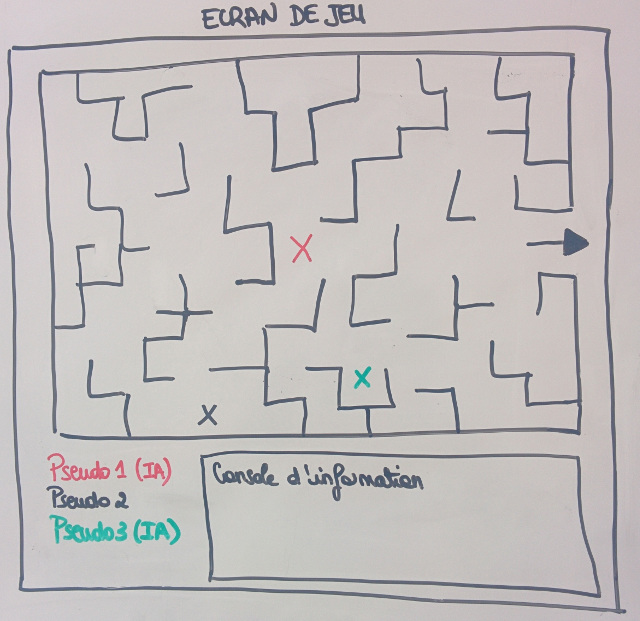
\includegraphics[width=15cm]{images/schema_ecran_partie.jpg}
		\caption{Schéma de l'écran d'une partie}
		\label{fig:ecran_partie}
	\end{figure}

	% ------------- Gestion des déplacements ------------
	\subsection{Gestion des déplacements}
	\label{subsec:gestion_deplacements}
	À chaque tour, un joueur dispose d'un temps limité pour indiquer son déplacement. Ce déplacement peut être: ``HAUT'', ``BAS'', ``GAUCHE'', ``DROITE''. À la fin du tour, le déplacement est effectué. On distingue deux manières de jouer: avec une IA ou sans IA\@.

	% ------------- Déplacement humain ------------
	\subsubsection*{Déplacement humain}
	Lorsqu'un joueur joue sans IA, il dispose d'un temps supérieur pour indiquer son déplacement. Il indique son déplacement à l'aide des touches fléchées. \color{red}Dans le cas où le joueur ne veut pas se déplacer, il peut appuyer sur la touche espace pour passer son tour.\color{black} Dans le cas où il n'appuie sur aucune touche avant la fin du temps imparti, il ne se déplace pas. Dans le cas où son déplacement n'est pas valide, par exemple si la destination est un mur, il ne se déplace pas non plus.

	% ------------- Déplacement avec une IA ------------
	\subsubsection*{Déplacement avec une IA}
	À chaque tour, l'IA dispose d'un temps pour indiquer son déplacement. Le programme indique son déplacement sous la forme d'une chaîne de caractère (``HAUT'', ``BAS'', ``GAUCHE'' ou ``DROITE''). Si la chaîne de caractère est mal formée, où si le programme met trop de temps à répondre, le joueur ne se déplace pas. De la même manière que pour les joueurs humains, si le déplacement n'est pas valide, il n'est pas pris en compte.
